\section{Auswertung}

In der folgenden Auswertung werden die verschiedenen aufgenommenen Spektren
ausgewertet, um die Eigenschaften des Detektors zu bestimmen so zwei verschiedene
unbekannte Quellen zu klassifizieren. Dafür werden verschiedene \textsc{Python}-Pakete
verwendet. Es handelt sich um die Pakete \textsc{uncertainties} für die Fehlerrechnung,
\textsc{scipy.optimize} für die Bestimmung der verschiedenen Peaks sowie
\textsc{curve\_{fit}} für die Ausgleichsrechnungen.

\subsection{Kalibrierung des Detektors mit einer $^{152}\ce{Eu}$-Quelle}
\label{subsec:Eu}

Zu Beginn des Experimentes wird eine Kalibrierung des Detektors mithilfe
einer $^{152}\ce{Eu}$-Probe durchgeführt. Anhand des Spektrums werden dann mithilfe
bekannter Energien des Gamma-Spektrums die Transformation der Kanäle in die
entsprechenden Energien sowie die Parameter für die Effizienz in Abhängigkeit
der Energie bestimmt. Die Messung wurde in einem Zeitraum von
$t\ua{ges} = \SI{3393}{\second}$ durchgeführt.

\subsubsection{Bestimmung der Energie-Transformation}

\begin{figure}
  \centering
  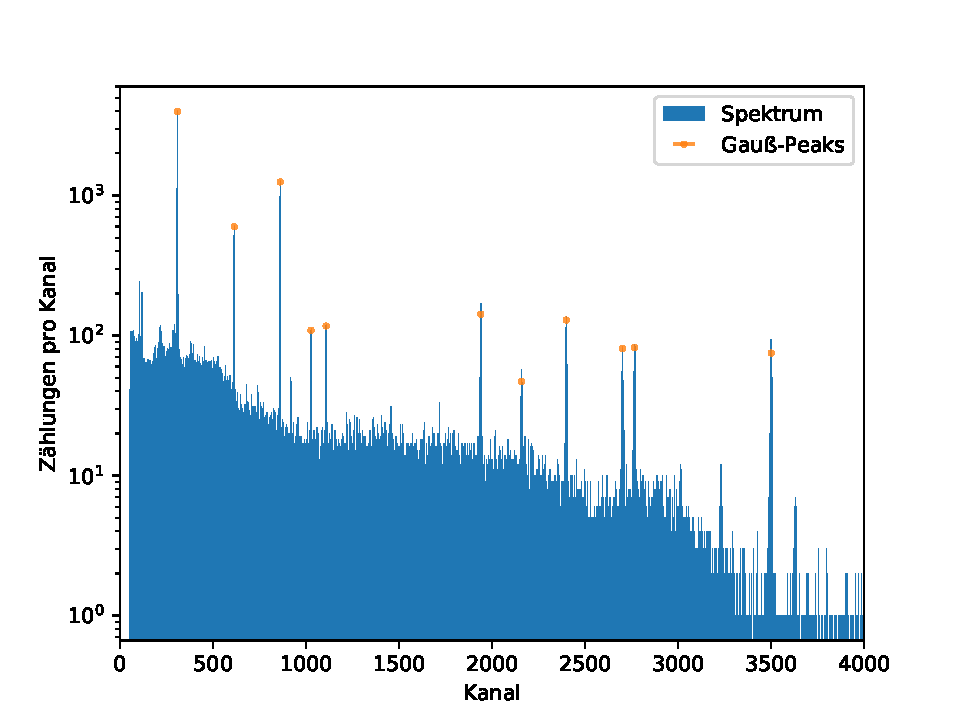
\includegraphics[width = 0.8\textwidth]{Python/Plots/Europium.pdf}
  \caption{}
  \label{fig:EuSpek}
\end{figure}
In Abbildung \ref{fig:EuSpek} ist das aufgenommene Spektrum für
$^{152}\ce{Eu}$ dargstellt. Um den einzelnen Kanälen eine Energie zuordnen
zu können, werden die Kanäle der verschiedenen Peaks mit \textsc{scipy.optimize.find\_{peaks}}
bestimmt. Anschließend wird jeweils in einem Bereich von $\pm \num{30}$ Kanälen
um die bestimmten Kanäle eine
Anpassung mit der folgenden Gauß-Funktion durchgeführt:
\begin{equation}
  N(x) = A\cdot exp{\left( \frac{x-\mu}{\sigma}\right)^2} + B.
  \label{eqn:Gausfit}
\end{equation}
Die einzelnen Parameter sind in Tabelle \ref{tab:EuGauß} eingetragen und die bestimmte
Mittelwerte der Peaks sind in Abbildung \ref{fig:EuSpek} dargestellt. Jedem
Peak wird dabei eine der charakteristischen Energien aus dem Gamma-Spektrum
von $^{152}\ce{Eu}$ zugeordnet. Mithilfe der gefitteten Mittelwerte $\mu$ kann
nun die Transformation der Kanäle in die zugehörigen Energiewerte bestimmt werden.
Dafür werden die Energien $E_{\gamma, \text{lit}}$ an die bestimmten Kanäle $\mu$ gemäß
einer linearen Funktion der Form
\begin{equation}
  E(x) = m \cdot x + b
\end{equation}
angepasst. Dabei ergeben sich die folgenden Parameter:
\begin{align}
  m &= \SI{0.40299(6)}{\kilo\eV\per\text{Kanalnummer}} \\
  b &= \SI{-2.76(11)}{\kilo\eV}
\end{align}
Die verwendeten Kanalnummern, die dazugehörigen Literaturwerte der Energien
$E_{\gamma, \text{lit}}$ sowie die mit der Transformation bestimmten Energien
$E_{\gamma}$ sind in Tabelle \ref{tab:Kalibrierung} eingetragen. In Abbildung
\ref{fig:Kalibrierung} sind die Datenpunkte sowie der dazugehörige Fit
grafisch dargestellt. Die bestimmten Parameter werden in den folgenden Abschnitten
verwendet, um das Spektrum direkt in Abhängigkeit von der Energie darzustellen.
\begin{figure}
  \centering
  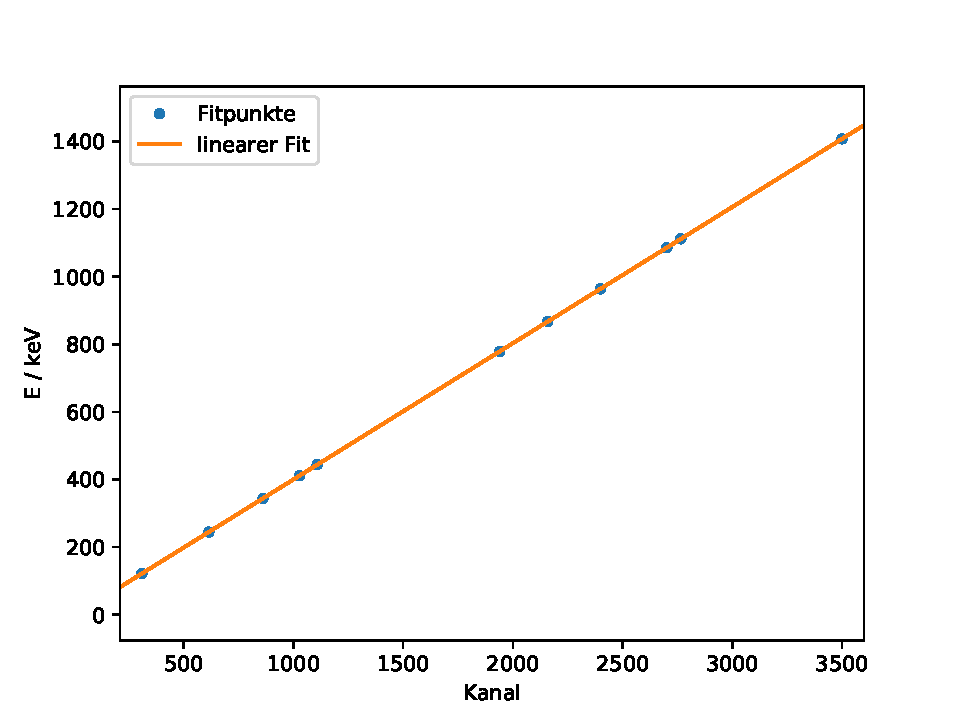
\includegraphics[width = 0.8\textwidth]{Python/Plots/Kalibrierung.pdf}
  \caption{}
  \label{fig:Kalibrierung}
\end{figure}

\subsubsection{Bestimmung der Parameter für die Effizienz}

Die Nachweiswahrscheinlichkeit der Gamma-Quanten ist im Allgemeinen von der Energie
abhängig, weshalb im folgenden eine Funktion für die Effizienz in Abhängigkeit von
der Energie bestimmt werden soll. Dafür muss zuerst die Aktivität der Probe
bestimmt werden. Es ist bekannt, dass die Aktivität der Probe am 01.10.2000
$A\ua{0} = \SI{4130(60)}{\becquerel}$ betrug. Bei einer Halbwertszeit von
$t\ua{1/2} = (\num{4943(5)})\,\text{Tagen}$ ergibt sich somit gemäß des Zerfallsgesetzes
für den 10.12.2018 eine Aktivität von $A=\SI{1627(24)}{\becquerel}$. Desweiteren
wird der Raumwinkel benötigt, den der Detektor abdeckt. Dieser kann gemäß Formel ??
bestimmt werden. Der Abstand zwischen Probe und Detektor beträgt $d = \SI{88.5}{\milli\meter}$
und der Detektor hat einen Radius von $r = \SI{22.5}{\milli\meter}$. Für den Raumwinkel
ergibt sich somit
\begin{equation}
  \frac{\Omega}{4\pi} = 0.0154
\end{equation}
Die Übergangswahrscheinlichkeiten werden der Quelle ?? entnommen und sind zusammen
mit den restlichen Werten sowie den bestimmte Effizienzen in Tabelle \ref{tab:Effizienz}
eingetragen. An die bestimmten Effizienzen wird eine Funktion der Form
\begin{equation}
  Q(E) = A\cdot E^{-B}
\end{equation}
angepasst. FÜr die beiden Parameter ergeben sich
\begin{align}
  A &= \SI{110(23)}{\per\kilo\eV} \\
  B &= \SI{1.07(3)}{}.
\end{align}
Die verwendeten Datenpunkte sowie die dazugehörige Fitfunktion sind in
Abbildung \ref{fig:Effizienz} dargestellt.
\begin{figure}
  \centering
  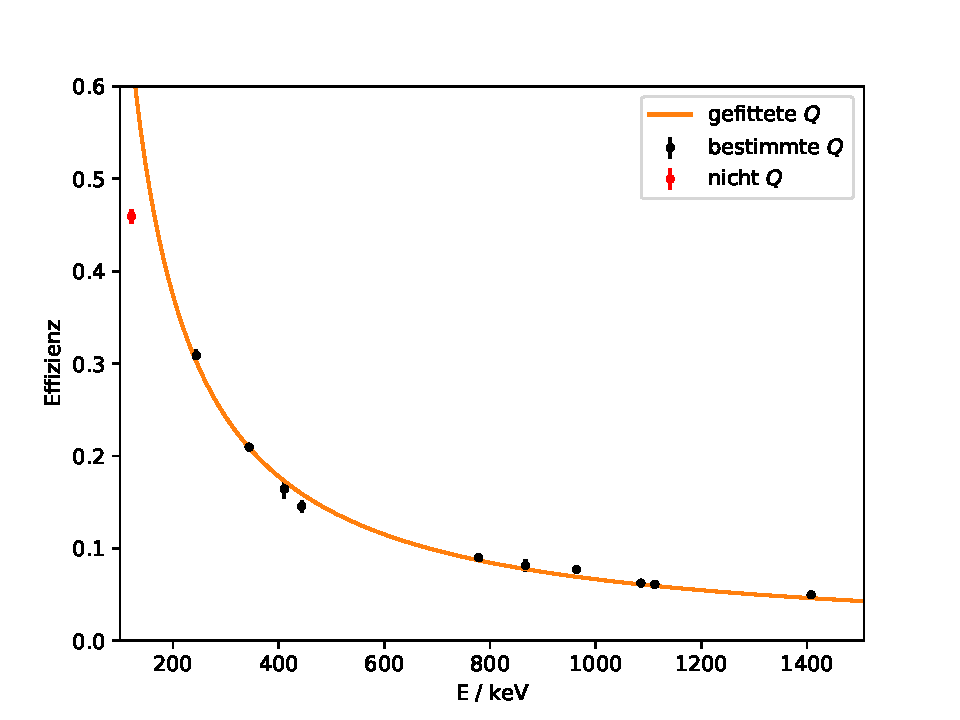
\includegraphics[width = 0.8\textwidth]{Python/Plots/Effizienz.pdf}
  \caption{}
  \label{fig:Effizienz}
\end{figure}

\subsection{Bestimmung verschiedener Detektoreigenschaften mithilfe einer $^{137}{Cs}$-Quelle }

Das aufgenommene Spektrum für $^{137}{Cs}$ ist in Abbildung \ref{fig:Ca} dargestellt.
Der Vollenergiepeak wurde analog zu Kapitel \ref{subsec:Eu} mithilfe des
\textsc{find\_{peaks}}-Paketes bestimmt und gemäß Formel \eqref{eqn:Gausfit}
angepasst. Dabei ergeben sich die folgenden Parameter:
\begin{align}
  A &= \SI{2054(13)}{Zählungen} \\
  \mu &= \SI{661.4(2)}{\kilo\eV} \\
  \sigma &= \SI{2.15(2)}{\kilo\eV} \\
  B &= \SI{6{3}}{Zählungen}.
\end{align}
Um die Verwendung einer Gauß-Funktion als Fitfunktion zu rechtfertigen, wird die
Halbwertsbreite sowie die Zehntelbreite bestimmt. Dafür werden die beiden Bins
gesucht, die die geringste Abweichungen zur Hälfte bzw. dem Zehntel der bestimmten
Amplitude haben. Für die Halbwertsbreite und Zehntelbreite sowie deren Verhältniss
ergibt sich somit:
\begin{align}
  x\ua{1/2} &= \SI{2.4(2)}{\kilo\eV} \\
  x\ua{1/10} &= \SI{4.4(2)}{\kilo\eV} \\
  \frac{x\ua{1/10}}{x\ua{1/2}} &= \SI{1.83(18)}{}.
\end{align}
